\subsection{Normal Log-PDF}

\begin{figure*}[t]
    \centering
    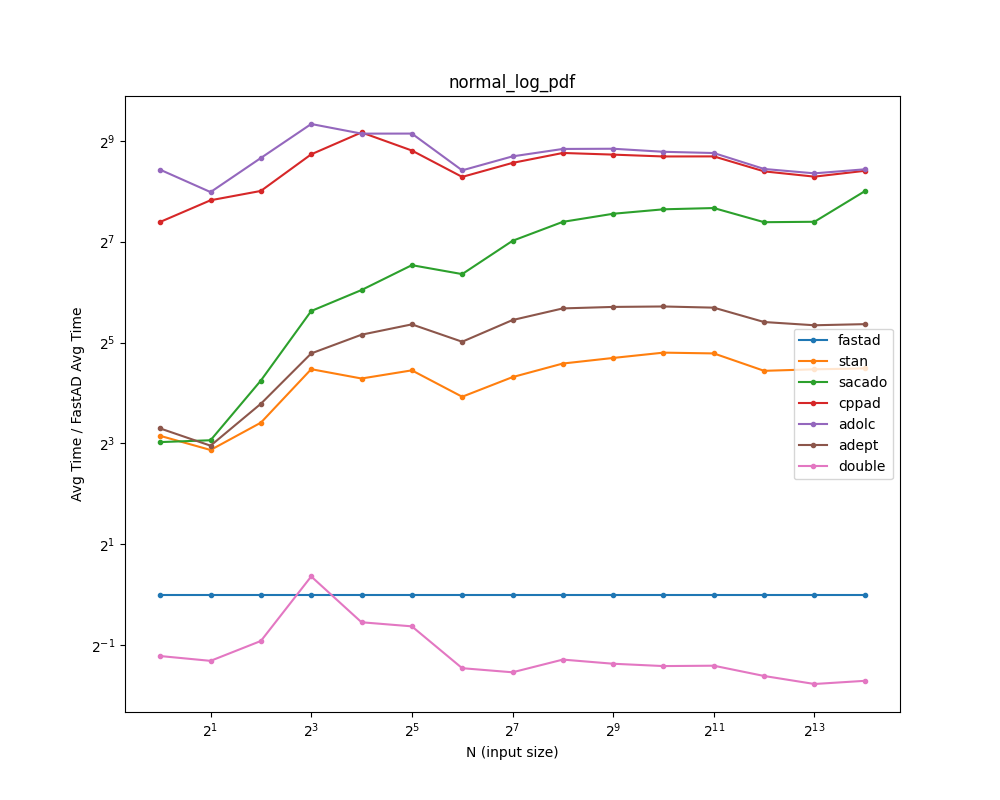
\includegraphics[width=0.8\textwidth]{figs/normal_log_pdf_fig.png}
    \caption{%
        Normal log-pdf benchmark of other libraries against FastAD 
        plotted relative to FastAD average time.
    }\label{fig:normal_log_pdf}
\end{figure*}

The normal log-pdf function is defined up to a constant:
\[
    f(x) = -\frac{1}{2\sigma^2} \sum\limits_{i=1}^N \paren{x_i - \mu}^2 
           -N\log(\sigma)
\]
For this benchmark, $\mu = -0.56,\,\sigma = 1.37$ and are kept as constants;
the values themselves are not so important so long as $\sigma > 0$
and are used consistently across all libraries.
Only Stan and FastAD provide built-in functions to compute this function.
Adept provides \code{norm2} function that computes squared-norm,
however, this did not produce the correct adjoints.
Hence, our only choice was to write a naive for-loop method.
Fig.\ref{fig:normal_log_pdf} shows the benchmark results.

FastAD is the fastest library for all values of $N$.
It is not surprising that Stan is the next fastest, 
since the Stan Math Library was written precisely for differentiating probability densities.
It is, however, surprising that Adept is the third fastest,
given that we wrote our own for-loop to implement its overload.
The trend stabilizes at around $N=2^{7}=128$.
Towards the end,
Stan is about $ 22$ times slower,
Adept about $ 41$ times,
and Sacado about $ 198$ times.
This difference is the largest we have seen so far,
and this is largely due to how we compute $\log(\sigma)$.
Section~\ref{ssec:normal_log_pdf} showed that when $\sigma$ is constant,
the compiler generates code to compute $\log(\sigma)$ only once
and gets reused over multiple AD evaluations with no other cost during runtime.
